\documentclass[11pt]{article}

\usepackage[]{graphics}
\usepackage{natbib}
\usepackage{rotating}
\usepackage[margin=2cm]{geometry}
\usepackage{pgfgantt}

\usepackage{csvsimple}

%opening
\title{Developing an Intelligent Chatbot: the First Interim Report}
\author{Group xx: Daniel Willis, Charlotte Anderson and Brandon Gous}

\begin{document}
	
	\maketitle	
	\begin{abstract}
		This interim report presents (1) the outline of our coursework report, (2) some initial descriptions of the requirements of the coursework, the methods, programming languages, packages, tools that have been identified so far, and (3) an initial work plan.
	\end{abstract}
	
	\section{Introduction}
	
	%(Brief introduction to the coursework. You don't have to write much.  
	%You may introduce a bit on chatbot in general if like, and why an intelligent chatbot is useful using the subsections headings if you wish.) 
	
	For this coursework we are developing a chatbot to help customers in finding the cheapest available ticket for their chosen journey also to improve customer service satisfaction by applying some appropriate AI techniques.
	
	\subsection{Background and Motivation}
	A bit background information on chatbot in general and the coursework specification\citep{AI2018CW}.
	
	\subsection{Aim and Objectives of this coursework} 
	You may rephrase the the aim and objectives from your point of view.  
	
	\subsection{Difficulties and Risks}
	
	List as many as you can identify. 
	
	\subsection{Work Plan}	
	
	\begin{figure}{Project Gantt chart \label{pplan}}
			\begin{ganttchart}[x unit=0.35cm, y unit chart = 1.0cm, y unit title=0.5cm, title height=1.0, vgrid, title label font=\scriptsize,
				canvas/.style={draw=black, dotted},
				/pgfgantt/milestone left shift = 0,
				/pgfgantt/milestone right shift = 0
				]{6}{18}
				
				\gantttitle{Project schedule week numbers}{13} \\
				\gantttitlelist{6,...,18}{1}\\
				\gantttitlelist{6,...,12}{1}
				\gantttitle{CB}{4}
				\gantttitle{AP}{2}\\
				
				\ganttbar{Asses what needs to be done}{6}{8}\\%elem0  
				\ganttbar{Design}{8}{9}\\%elem0
				\ganttbar{Create Scraper}{10}{11}\\%elem0	
				\ganttbar{Predictive Models}{10}{13}\\%elem0
				\ganttbar{Create UI}{12}{12}\\%elem0	
				
				\ganttbar{Create Knowledge Base}{13}{14}\\%elem0	
				\ganttbar{Develop Natural Language Processing}{13}{14}\\%elem0	
							
				\ganttbar{Report Writing}{7}{8}
				\ganttbar{}{15}{17}\\%elem0		
				
						
				\ganttmilestone{Progress Check}{12}\\%elem8 
				\ganttmilestone{Due Date}{17}\\%elem8  
				
				\ganttlink{elem0}{elem1}				\ganttlink[link mid=.25]{elem1}{elem2}
				\ganttlink[link mid=.25]{elem1}{elem3}
				\ganttlink{elem2}{elem4}
			\end{ganttchart}
	\end{figure}
	\section{Related Work} 
	Review some similar chatbot systems. (Write as much as you have now.)  
	
	\section{Methods, Tools and Frameworks}
	In this section, you should describe the methods, programming languages, packages, tools and framework you plan to use.
	for this report, you can list some you have identified and intend to use.
	No need to give any details.     
	
	\subsection{Methods}
	
	You may list some methods you will use for developing your chatbot, including 
	
	Such as what type of user interface (graphical, text, or voice, etc) you intend to use.
	
	What Natural Language Processing and understanding methods you intend use, 
	
	What referring or reasoning methods
	
	What prediction methods, such as kNN, neural networks etc. 
	
	\subsection{Languages, Packages, Tools}
	
	On programming language: using Python or Java, or others. 
	
	Packages: for NLP, use NLTK\citep{NLTK}, or others, 
	
	For KnowledgeBase and Engine: PyKE or PyKnow, or others. 
	
	For Database: e.g, Postgres, or MongoDB     
	
	\subsection{Development Framework}
	
	
	\section{Design of the Chatbot}	
	
	\subsection{The Architecture of the chatbot}
	You may draw a functional diagram if you like.  
	
	You can describe your design for each key module or component of your chatbot, in a subsection. E.g. 
	\subsection{User Interface} 
	
	\subsection{NLP}
	
	\subsection{Knowledgebase}
	
	\subsection{Inferring Engine}
	
	\subsection{Delay Prediction Models}
	
	For our prediction models we implemented three. A Bayesian model that calculated the probability of the train being late to the second station given that the train is delayed to the first station. A neural network that uses the delay and the normal time it takes between the stations to predict how late the train will be. And K nearest neighbour which predicts how late the train will be to the second station.
	
	\subsubsection{Bayesian}
	
	Bayesian Theorm is that the probability of event A happened given that B happened can be calculated by the probability of event B happening given that event A happened multiplied by the probability of event A happening all divided by the probability of event B happening.	
	\[P(A|B) = (P(B|A) * P(A))/P(B)\]
	
	Additionally this can be expanded so that the probability of event B happening doesn't need to be known. The probability of event B happening is equal to the probability of event B happening given event A happened multiplied by the probability of event A occurring plus the probability of event B happening given that event A does not multiplied by the probability that event A does not happen.
	
	\[P(B) = P(B|A) * P(A) + P(B|'A) * P('A)\]
	
	This means that you can calculate the probability of event A happening given that B happened from the probability of event A happening, the probability of  event B happening given event A happened and the probability of event B happening given that event A didnt happen.
	\[P(A|B) = (P(B|A) * P(A))/(P(B|A) * P(A) + P(B|'A) * (1 - P(A)))\]	
	
	I applied this to the prediction of trains being late by making A the event of the train being late to the second station and B the event of the train being late by delay or more to the first station.
	
	To get these probabilities I used stored procedures to extract the frequencies from the database.
	
	Firstly the probability of A (the train being late to the second station). This was easy enough to calculate I simply extracted the frequency count of all times it arrived at the second station. Totalled up the number of times the train was late and divided by the total pieces of data I had.
	
	Secondly I calculated the probability of B given A. To do this I extracted the frequencies of delays at the first station if the train arrived late to the second station. From here I summed all the frequencies that the train was late to the first station by atleast the delay.
	
	Next I calculated the probability of B given not A. To do this I extracted the frequencies of delays at the first station if the train arrived on-time or early to the second station. From here I summed all the frequencies that the train was late to the first station by at least the delay.	
	
	\subsubsection{Neural Network}
	\subsubsection{K Nearest Neighbors}		
	
	For the K nearest neighbour model we have to use load of data extracted from the database for each query. To do this I used a stored procedure to get the amount that all the trains was late to both stations specified. 
	
	The amount the train was late to the first station is then compared to the amount of delay that the user had at the first station using a distance function, in my case picked euclidean.
	
	These distances are then sorted and you get the mean of the delay at the second station for the closest K nodes in the dataset. This is simple algorithm but heavily dependant on finding the correct K value.
	
	To find the best K value a set up a test to run one thousand iterations of selecting random data points from the data. Then for each piece of data I would create a KNN object with a different value of K ranging 1 to 100 (inclusive). Get a prediction from each object and compare it to the target outcome. From this I calculated the root mean square error for each value of K over the iterations.
	
	The results plotted on a graph is in figure \ref{Img:KSearch} and the top ranking results are included in the table in figure \ref{Img:KSearchRaw}.	
	The shape of the graph is exactly what I expected to see with very few neighbours having a very high RMSE and then having a dip where the ideal K value is with the RMSE gradually increasing again as the more neighbours are used.
	
	\begin{figure}[!htb]
		\begin{center}
			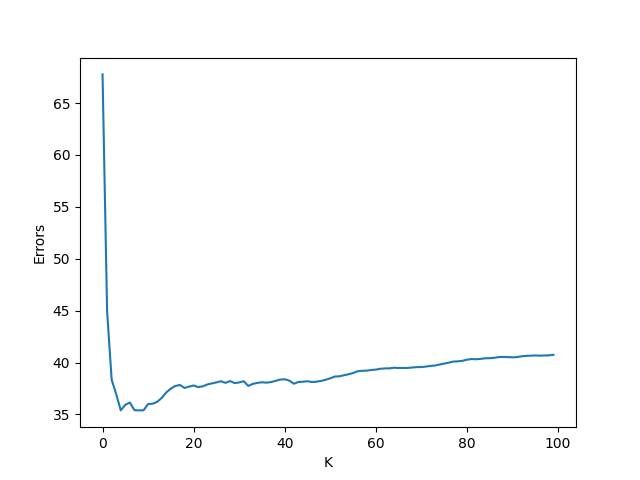
\includegraphics[width=1.2\textwidth]{Resources/PartTwo/searchingForK_20220110_065714.png}
			\caption{Searching for the correct K value}
			\label{Img:KSearch}
		\end{center}
	\end{figure}
	
	\begin{figure}[!htb]
		\begin{center}
				\csvautotabular{Resources/PartTwo/KResults_Sorted.csv}
			\caption{Sorted RMSE of K values}
			\label{Img:KSearchRaw}
		\end{center}
	\end{figure}

	From these results I concluded that 9 was the best value for K not only because it ranks at the top but because 10 and 8 rank 3rd and 4th in the list. However any value from 5 - 15 would be very accurate still.
	
	\subsubsection{Comparison}
	I didn't think that the Bayesian model was very good it is more of a classification model not a regression therefore not particularly useful.
	
	\begin{figure}[!htb]
		\begin{center}
			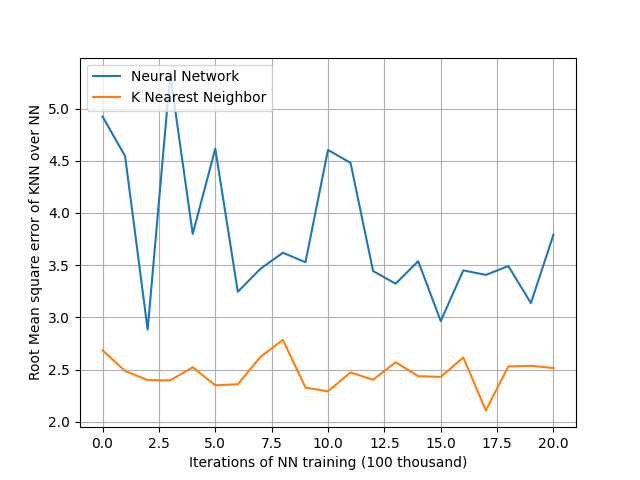
\includegraphics[width=1.2\textwidth]{Resources/PartTwo/Comparison_20220112_152958.png}
			\caption{Comparison of neural network and K nearest neighbour}
			\label{Img:NNKNNComp}
		\end{center}
	\end{figure}
	
	In figure \ref{Img:NNKNNComp} below I compare the neural network and k nearest neighbours over two million iterations of training the neural network.
	
	This was accomplished by randomly selecting a thousand data sets, running these datasets through both the models and comparing the predictions to the targets. Then train the neural network on the same dataset for a hundred thousand iterations and repeat.
	
	As you can see the K nearest neighbour algorithm is consistently better than the neural network despite the improvements made so we decided to use that.		
	
	\subsection{Conversation Control}
	
	%\begin{table}
		%\centering
		%\caption{This table lists ......}
		%
		%\begin{tabular}{|c|c|c|c|c|c|}
			%\hline Methods &  &  &  &  &  \\ 
			%\hline  &  &  &  &  &  \\ 
			%\hline  &  &  &  &  &  \\ 
			%\hline 
			%\end{tabular} 
		%\label{TableCC}
		%\end{table}
	
	\section{Implementation}
	
	\section{Testing}
	
	\subsection{Unit Testing}
	
	\subsection{Integration Testing}
	
	\subsection{System Testing}
	
	\subsection{Userbility Testing}
	
	\section{Evaluation and Discussion}
	
	\section{Conclusion or Summary}
	
	\bibliographystyle{agsm}
	%\bibliographystyle{apalike}
	% you should use your own bibtex file to replace the following example_ref bib file.
	\bibliography{example_refs} 
	
\end{document}
